% !TEX root = ../main.tex
\chapter{Technical Background}
\label{ch:techbackground}
\section{Machine Learning}
\label{sec:bg1}

\subsection{Artificial Neural Networks}
Artificial neural networks (ANN) form the basis for the machine learning models that will be used for predicting states and making trading decisions. An ANN consists of layers of nodes connected to one another. Each node produces an output based on the inputs to the node and the tuning parameters; weights and biases. A neural network consists of:
\begin{itemize}
    \item Input Layers: Holds the raw input to the system. For example, the RRP in the NEM for the previous 24 hours.
    \item Hidden Layers: Consist of nodes that transform inputs into new representations using linear transformation. 
    \item Output Layers: Transform the output from the hidden layers to a final state using the nonlinear activation function. For example, the predicted RRP in the NEM.
\end{itemize}

\begin{figure}[H]
    \centering
    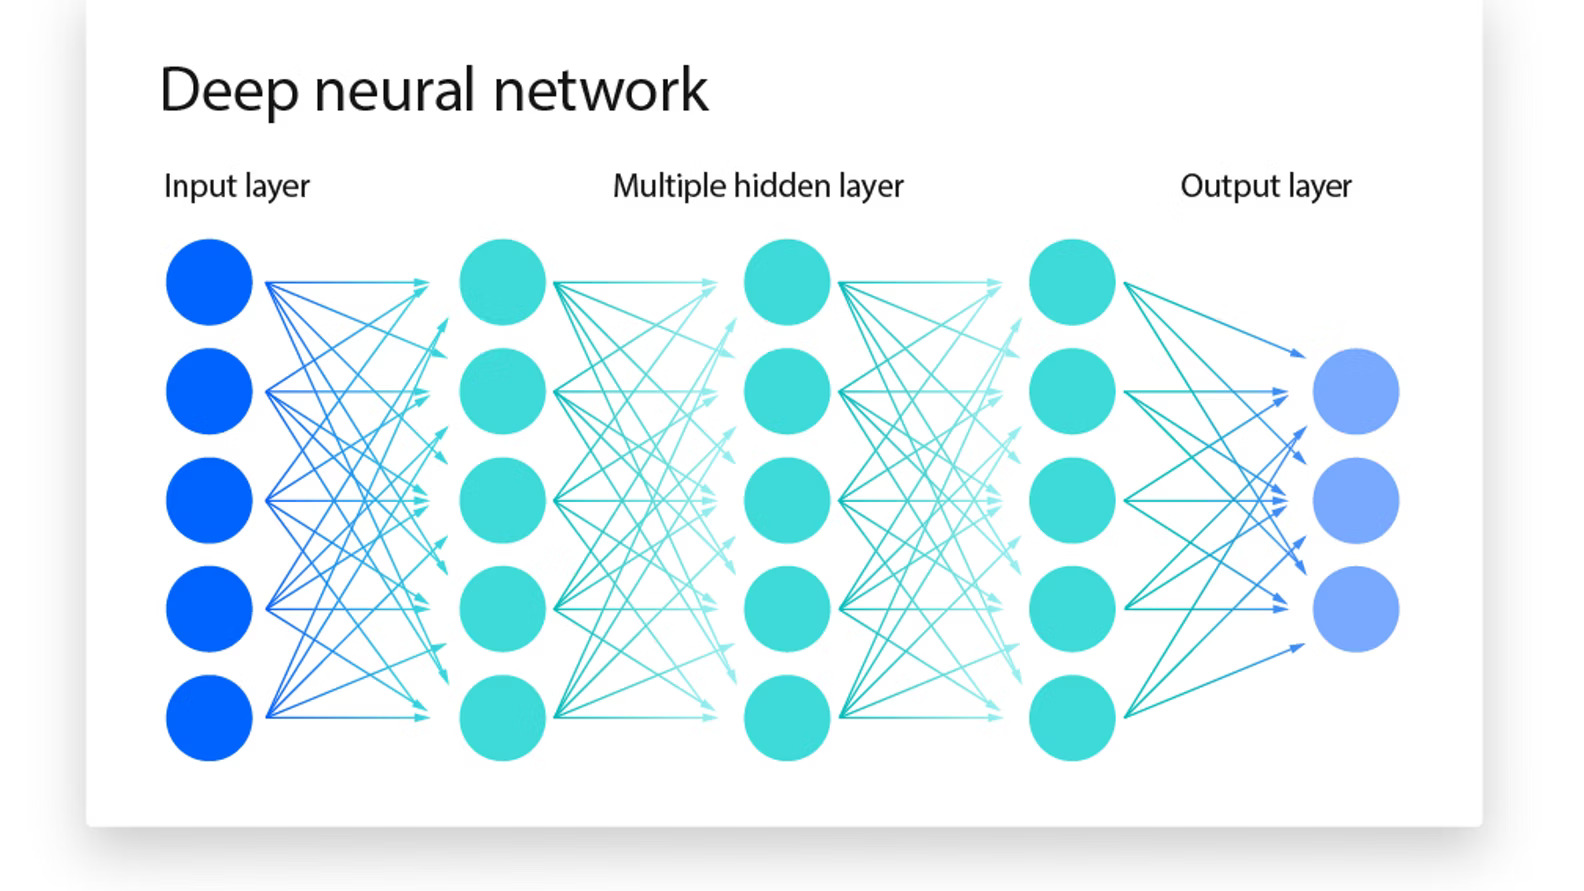
\includegraphics[width=0.8\textwidth]{images/DeepNeuralNetwork.jpg}
    \caption{A standard feedforward neural network with 3 hidden layers \cite{lee_neural_networks_ibm}.}
    \label{fig:neural_network}
\end{figure}

A single neuron computes a weighted sum , $z$, and an output, $a$ \cite{lee_neural_networks_ibm}: \par

\begin{equation}
      z = \sum_{i=1}^{n} w_i x_i + b
\end{equation}
\begin{equation}
            a = \sigma(z)
\end{equation}
Where
\begin{itemize}
  \item $x_i$ = input feature,
  \item $w_i$ = weight,
  \item $b$ = bias,
  \item $\sigma$ = activation function (nonlinear transformation),
\end{itemize}

The weights and biases of the ANN are adjusted through comparing the network’s prediction, $\hat{Y}$, to the true label, $Y$, and measuring the error using a loss function. To minimise this loss function, backpropagation is used to train the neural network. Backpropagation consists of four steps:
\begin{enumerate}
    \item Forward pass: Inputs flow through the network, computing outputs at each node and producing an output prediction.
    \item Error calculation: The error between the expected and actual output is calculated using the loss function.
    \item Backward pass (back propagation): The error is propagated back through the network. For each neuron the algorithm calculates the contribution of the weight and bias to the error using the chain rule of calculus.
    \item Weight update: Using gradient descent methods, the weights and biases are adjusted slightly to reduce the error.
\end{enumerate}

This process is repeated many times over a training set to tune the internal parameters of the network. With appropriate training the network converges to minimise the loss function. An example for this project would be the minimisation of error for predicting NEM RRP.

\subsection{Long Short Term Memory}
Long Short Term Memory (LSTM) networks are a type of recurrent neural network (RNN) designed by Hochreiter and Schmidhuber \cite{Hochreiter1997}. RNNs are commonly used ML models for state prediction such as price forecasting. They contain a specific type of neuron called a  recurrent neuron. Recurrent neurons have a hidden state that holds information about the previous inputs. Through using Backpropagation Through Time (BPTT), the weights of the network are updated to minimise error across timestamps.

LSTM introduces a memory cell that holds information over extended periods. This acts as long-term memory for the network and assists with pattern recognition. Each memory cell has three gates:
\begin{itemize}
    \item \textbf{Input Gate:} Controls the information added to the memory cell.
    \item \textbf{Forget Gate:} Determines what information is removed from memory cell.
    \item \textbf{Output Gate:} Controls information output from memory cell.
\end{itemize}


\subsection{Reinforcement Learning}
This project will consider a Reinforcement Learning (RL) approach for controlling household battery operation. RL has shown benefits over MILP when considering the non-linear characteristics of battery degradation and charging efficiencies. The model will take in predicted states, $\hat{G}, \hat{A}, \hat{P}$, and output an action.

\subsubsection{Markov Decision Process}
\label{sub:sub:Markov}
A Markov decision process (MDP) is a mathematical model for sequential decision making when outcomes are uncertain. It is a method to define the problem the RL model will navigate. A MDP is defined by several properties \cite{cs188_mdp_2024}:
\begin{itemize}
    \item A set of states, $S$.
    \item A set of actions, $A$.
    \item A start and terminal state(s).
    \item A transition function, $T(s, a, s')$. Actions in an MDP may be nondeterministic; the transition function represents the probability of an agent taking an action $a \in A$ from a state $s \in S$ and ending up in a state $s' \in S$.
    \item A reward function, $R(s,a,s')$. This reward may be positive or negative.
\end{itemize}

Figure~\ref{fig:MDP} illustrates a basic MDP with three states. The transition function is represented by the probabilities indicated on each action branch and the agent is rewarded based on the states visited. We define the optimal policy function to minimise the expected cost to the goal as $\pi$.

\begin{figure}[h]
    \centering
    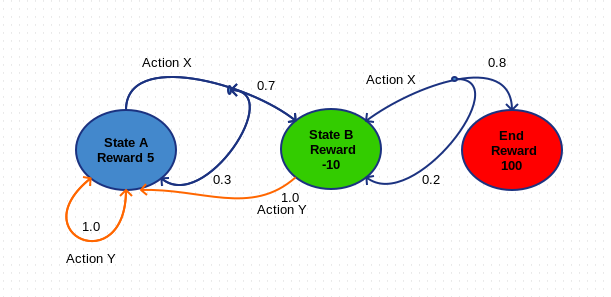
\includegraphics[width=0.8\textwidth]{images/MDP.png}
    \caption{A basic MDP \cite{yale_cs470_mdp}}
    \label{fig:MDP}
\end{figure}



\subsubsection{Dynamic Programming and Bellman Equations}
Dynamic programming (DP) is a systematic technique for finding optimal policies of an MDP through solving the Bellman equation. The Bellman equation expresses the optimal value of being in a state as the immediate reward available plus the discounted optimal value of the next state. Solving the Bellman Equation requires full knowledge of the environment and state transitions, this is called a model-based approach.
The Bellman equation can be defined as \cite{ljungqvist_sargent_2004}:
\begin{equation}
    V^*(s) = \max_{a} \left[ R(s, a) + \gamma V^*(s') \right]
    \label{eq:bellman}
\end{equation}
where:
\begin{itemize}
    \item $V^*(s)$ is the optimal value of being in state $s$
    \item $a$ is the action taken
    \item $R(s, a)$ is the immediate reward from taking action $a$ in state $s$
    \item $\gamma \in [0,1]$ is the discount factor, weighting future rewards relative to immediate rewards
    \item $s'$ is the next state resulting from action $a$
    \item $V^*(s')$ is the optimal value of the next state $s'$
\end{itemize}

\subsubsection{Training Overview - Model Based}
Model based reinforcement learning is developed as a Markov decision process with complete knowledge of the environment. A function $G$ is defined to denote the discounted return, and is defined as the sum of future discounted rewards:
 
\begin{equation}
    G = \sum_{t=0}^{\infty} \gamma^t R_{t+1} = R_1 + \gamma R_2 + \gamma^2 R_3 + \cdots,
\end{equation}

where:
\begin{itemize}
    \item $R_{t+1}$ is the reward for transitioning from state $S_t$ to $S_{t+1}$
    \item $0 \leq \gamma < 1$ is the discount rate.
\end{itemize}

Since $\gamma < 1$, rewards in the distant future are weighted less than rewards in the immediate future. The goal of the algorithm is to find a policy that will maximise the expected value of $G$ ($\pi*$). This is achieved through \cite{sutton2018reinforcement}: \par

\begin{itemize}
    \item \textbf{Policy Evaluation}: Applies the Bellman equation iteratively across all states until the value function converges to a steady value. Beginning from an arbitrary initialisation, each sweep updates the value of every state using the current estimates of neighbouring states.
   
    \item \textbf{Policy Improvement}: Constructs a new policy from the current value function. At every state, the greedy action is chosen to maximise $G$. The Policy Improvement Theorem guarantees the new policy is at least as good as the old one for all states.
    
    \item \textbf{Generalised Policy Iteration}: Alternates between these two steps, evaluating the current policy and improving it. This continues until the value functions converge and the policy is optimal.
\end{itemize}


\subsubsection{Monte Carlo Methods}
Monte Carlo methods are based on a model-free approach to RL where there is not complete knowledge of the environment. Monte Carlo methods learn from the experience of interacting with the environment. They sample and average returns from each state-action pair. Monte Carlo methods use an adapted generalised policy iteration where instead of computing value functions, value functions are learnt. As more returns are observed, the average converges to the expected value. These returns are only used after the agent arrives at the terminal state.
\cite{sutton2018reinforcement}.

\subsubsection{Temporal-Difference}
Temporal-difference (TD) learning combines aspects of Monte Carlo and DP. Like Monte Carlo methods, TD works without a model of the environment through learning from the agent's interactions. Similar to DP, TD methods update estimates during state transitions before reaching the terminal state in a process called bootstrapping. Bootstrapping can greatly increase the speed of learning, particularly in environments with long episodes. \cite{sutton2018reinforcement}

\subsubsection{Sarsa: On-Policy TD Control}
In on-policy TD control, the first step is to learn an action-value function rather than a state-value function. We define the action-value function as $q_{\pi}(s, a)$ for the current behaviour policy $\pi$ and for all states $s$ and actions $a$. Action-value pairs are updated after every transition from a non-terminal state $S_t$ as defined in Equation~\ref{eq:sara}. Whilst estimating the state-action pairs, we continually update the policy $\pi$ towards greediness with respect to $q_\pi$. \cite{sutton2018reinforcement}
\begin{equation}
    \label{eq:sara}
    Q(S_t, A_t) \leftarrow Q(S_t, A_t) + \alpha \left[ R_{t+1} + \gamma Q(S_{t+1}, A_{t+1}) - Q(S_t, A_t) \right]
\end{equation}

\subsubsection{Q-Learning: Off-Policy TD Control}
In Q-learning, the learned action-value function, $Q$, approximates the optimal action-value function independently of the policy being followed as defined in Equation~\ref{eq:qlearning}. \cite{sutton2018reinforcement}

\begin{equation}
    \label{eq:qlearning}
    Q(S_t, A_t) \leftarrow Q(S_t, A_t) + \alpha \left[ R_{t+1} + \gamma \max_{a} Q(S_{t+1}, a) - Q(S_t, A_t) \right]
\end{equation}

The policy will determine which state-action pairs are visited and updated however the update target always uses $max_{a} Q(S_{t+1}, a)$, meaning Q-learning converges to the optimal action-value function regardless of the policy being followed. \cite{sutton2018reinforcement}

\subsubsection{Deep Q-Learning}
Deep Q-Networks (DQN) combines Q-learning and neural networks. It additionally introduces experience replay and target networks. A visual representation of a DQN is shown in Figure~\ref{fig:dqn} and its features can be summarised as:
\begin{itemize}
    \item The network approximates the Q-value function $Q(s, a:\theta)$ where $\theta$ represents the trainable parameters. 
    \item A replay buffer stores past experiences in the DQN $(s, a, r, s')$.
    \item A target network with parameters $\theta^-$ is used but updated less frequently to prevent instability in parameters shifting too quickly.
    \item A loss function, Equation~\ref{eq:dq_loss}, that measures the difference between predicted and target Q-Values. 
    
    \begin{equation}
    \label{eq:dq_loss}
    L(\theta) = \mathbb{E} \left[ \left( R_{t+1} + \gamma \max_{a'} Q(S_{t+1}, a'; \theta^{-}) - Q(S_t, A_t; \theta) \right)^2 \right]
\end{equation}
\end{itemize}

\begin{figure}[H]
    \centering
    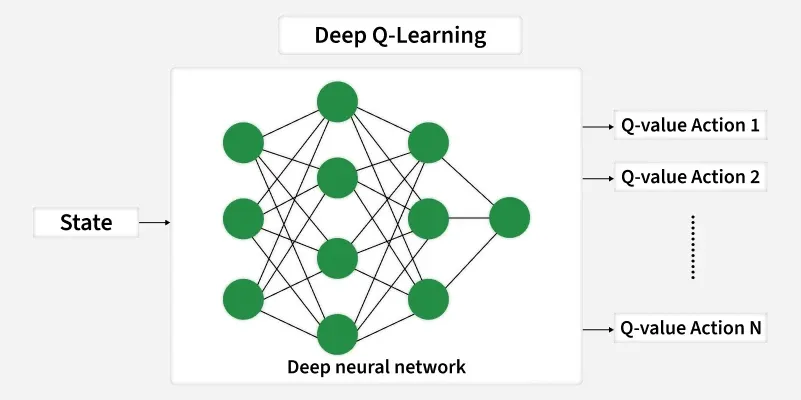
\includegraphics[width=0.8\textwidth]{images/deep_q_learning.png}
    \caption{Deep Q-Network \cite{geeksforgeeks_dqn_2025}}
    \label{fig:dqn}
\end{figure}




\section{Mixed Integer Linear Programming}
Linear programming (LP) involves the optimisation of a linear objective function subject to equality and inequality constraints \cite{Dantzig1963}. This can be expressed generally as:

\begin{align}
& \text{Find a vector} & & \mathbf{x} \notag \\
& \text{that maximizes} & & \mathbf{c}^\top \mathbf{x} \notag \\
& \text{subject to} & & A\mathbf{x} \leq \mathbf{b} \notag \\
& \text{and} & & \mathbf{x} \geq \mathbf{0} \notag
\end{align}

Mixed integer linear programming (MILP) extends this optimisation but restricts some or all of the variables to take integer values \cite{NemhauserWolsey1988}. This presents an alternative to RL for optimising the operation of the household battery. 

\subsection{Branch and Bound Algorithms}
Branch and bound algorithms are commonly used by solvers to discover the optimal solution for integer linear programs. The algorithm involves three steps \cite{LandDoig1960}:

\begin{enumerate}
  \item \textbf{Bounding}: At any node on the tree, the problem is relaxed to allow for non-integer solutions. This solution acts as the upper bound (for maximisation problems) of the objective value that can be achieved.
  
  \item \textbf{Branching}: From the relaxed solution two branches are created. A fractional variable $x_j$ is selected from the relaxed solution 
$x^*$, where $x_j^*$ denotes its relaxed value. One branch adds the constraint $x_j \geq \lceil x_j^* \rceil$ 
and the other adds $x_j \leq \lfloor x_j^* \rfloor$. The relaxed LP is then solved again.
 
  
  \item \textbf{Pruning}: Pruning involves the removal of branches from the algorithm. There are three types of pruning in branch and bound algorithms. 
  \begin{itemize}
  \item[--] Bound pruning: if the relaxed solution found at a node is worse than the best integer solution found, the branch is pruned.
  \item[--] Infeasibility pruning: if the relaxation of the subproblem is not feasible, due to the branching constraints rendering the feasible region empty, the branch is pruned.
  \item[--] Integer pruning: if the relaxed solution produces an integer value, update the incumbent value and prune.
\end{itemize}
\end{enumerate}


\section{System Characteristics}
\subsection{Network Tariffs}
Network tariffs are charged by electricity distributors to retailers for delivering electricity. The charge is associated with the infrastructure costs, maintenance, and operation of electricity transmission. Network infrastructure in NSW is a regulated asset, owned by private companies that are entitled to fixed revenue set by the Australian Energy Regulator \cite{AER_ReturnOnAssets}. This project will consider low-voltage residential connections on the Ausgrid network. This tariff consists of a daily metering service and network access charge along with a network energy price of 10.8007 cents/kWh \cite{ausgrid2024networkpricelist}.

\subsection{Battery and Inverter Models}
There is a wide variety of residential batteries available in the Australian market. Under the Small-scale Renewable Energy Scheme introduced in July 2025, the average nominal battery size has been 19.0 kWh \cite{CER2025battery}. This project will consider the specifications of the Tesla Powerwall 3. The Powerwall 3 is ubiquitous in home energy storage and has an inverter built into the battery system. The key technical specifications are summarised in the Table~\ref{tab:powerwall3_specs} \cite{tesla2025powerwall3}.

\begin{table}[h]
    \centering
    \caption{Tesla Powerwall 3 Technical Specifications}
    \label{tab:powerwall3_specs}
    \begin{tabular}{ll}
        \toprule
        \textbf{Parameter} & \textbf{Value} \\
        \midrule
        \multicolumn{2}{l}{\textit{Energy \& Power}} \\
        Usable energy capacity & 13.5 kWh \\
        Max.\ continuous discharge power & 11.04 kW\textsubscript{AC} \\
        Max.\ continuous charge power & 5 kW\textsubscript{AC} \\
        \midrule
        \multicolumn{2}{l}{\textit{Efficiency}} \\
        Solar to Battery to Home/Grid Efficiency & 89\% \\
        Solar to Home/Grid Efficiency & 97.5\% \\
        \midrule
        \multicolumn{2}{l}{\textit{Scalability}} \\
        Usable energy capacity per expansion unit & 13.5 kWh \\
        Expansion units per Powerwall 3 & Up to 3 \\
        Max.\ system energy capacity & 54 kWh \\
        \midrule
        \multicolumn{2}{l}{\textit{Solar Integration}} \\
        Maximum Solar STC Input  & 20 kW\textsubscript{DC} \\
        \bottomrule
    \end{tabular}
    \\ \vspace{0.5em}
\end{table}


\subsection{Cycle Depth Stress Function}
\label{sec:stressfn}
The degradation model of Section~\ref{sec:degradation} requires a cycle depth stress function $\Phi(\delta)$ and a replacement cost $R^{\text{cell}}$ to evaluate the marginal aging costs $c_j$ in \eqref{eq:goal:cj}. Xu et al.\ \cite{Xu2018} fit a near-quadratic stress function to Li(NiMnCo)O\textsubscript{2} 18650 cells:

\begin{equation}
    \label{eq:stressfn}
    \Phi(\delta) = (5.24\times10^{-4})\,\delta^{2.03}
\end{equation}

The exponent greater than unity is what makes the marginal cost curve convex, and hence what makes deep cycling progressively more expensive per unit of energy than shallow cycling.

Equation~\eqref{eq:stressfn} is adopted as an initial parameterisation, with the caveat that it is fitted to NMC chemistry, whereas the Powerwall 3 uses lithium iron phosphate (LFP). LFP cells exhibit a flatter relationship between cycle depth and life, so \eqref{eq:stressfn} is expected to overstate the penalty on deep cycling for this battery. Refitting the exponent against published LFP cycle life data, and quantifying the sensitivity of dispatch to that exponent, is identified as a task in Section~\ref{sec:bess_only}. The efficiencies $\eta^c$ and $\eta^d$ are taken as $\sqrt{0.89} \approx 0.943$ each, since Table~\ref{tab:powerwall3_specs} reports a round trip figure.

\subsection{Solar}
The average solar installation size has continued to increase. In the first quarter of 2025, the average installation size in NSW was 9.9 kW \cite{AEC2025Solar}.
